\subsection{RBC tumbling and tank-treading}

\begin{figure}[thb]
    \centering
    \begin{subfigure}{\textwidth}
    \begin{minipage}{0.2\textwidth}
        \centering
        \topinset{(a)}{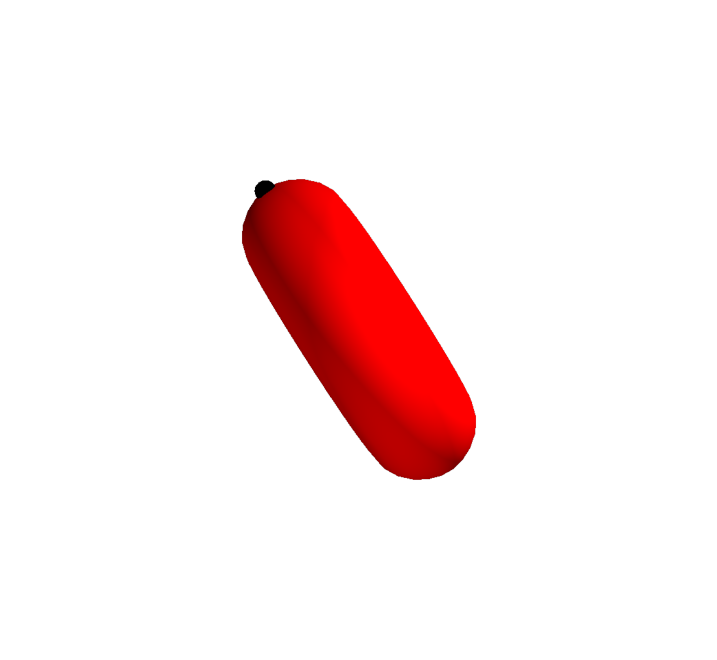
\includegraphics[trim=75 100 75 100, clip, width=\textwidth]{figures/tumble0000.png}}{0.5cm}{0.25cm}\\
        $\dot{\gamma}t = 0$
    \end{minipage}%
    \begin{minipage}{0.2\textwidth}
        \centering
        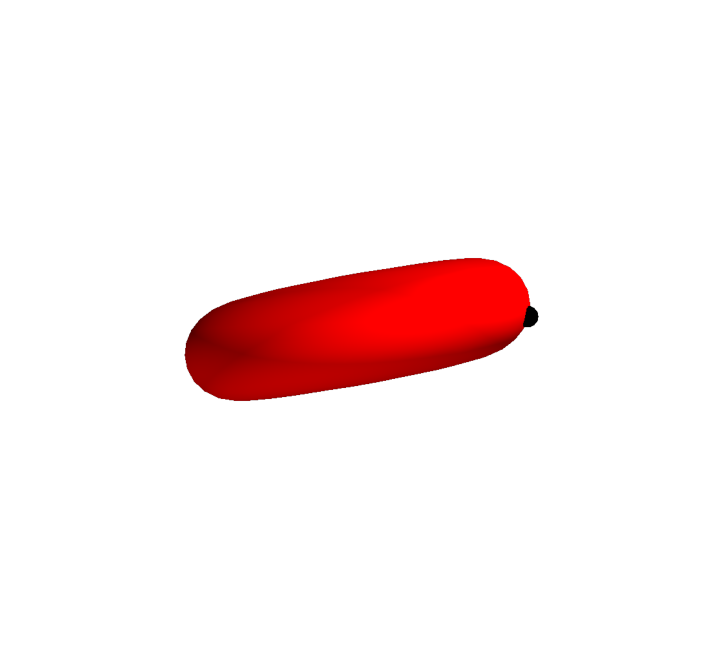
\includegraphics[trim=75 100 75 100, clip, width=\textwidth]{figures/tumble1000.png}\\
        $\dot{\gamma}t = 5$
    \end{minipage}%
    \begin{minipage}{0.2\textwidth}
        \centering
        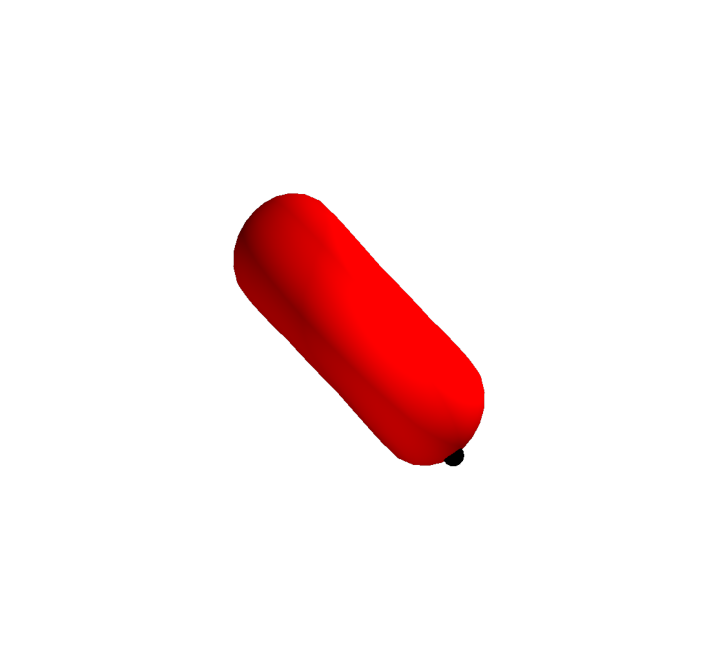
\includegraphics[trim=75 100 75 100, clip, width=\textwidth]{figures/tumble2000.png}\\
        $\dot{\gamma}t = 10$
    \end{minipage}%
    \begin{minipage}{0.2\textwidth}
        \centering
        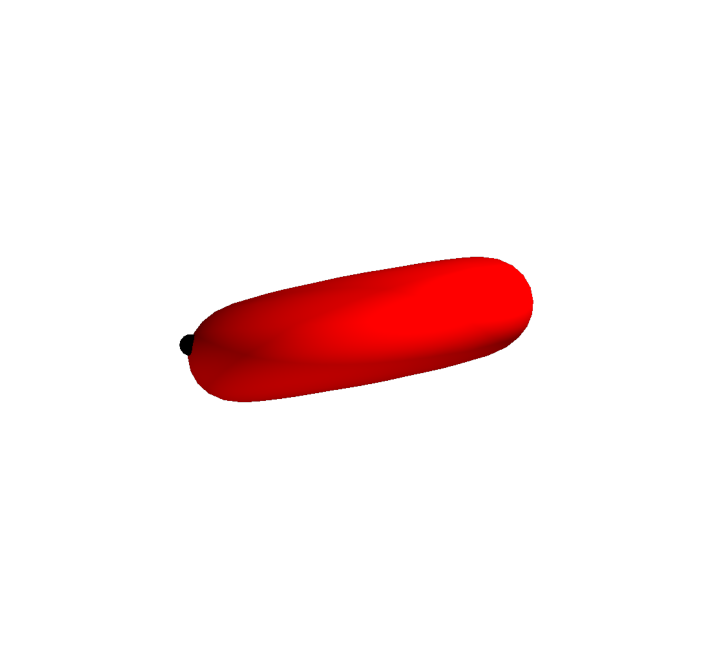
\includegraphics[trim=75 100 75 100, clip, width=\textwidth]{figures/tumble3000.png}\\
        $\dot{\gamma}t = 15$
    \end{minipage}%
    \begin{minipage}{0.2\textwidth}
        \centering
        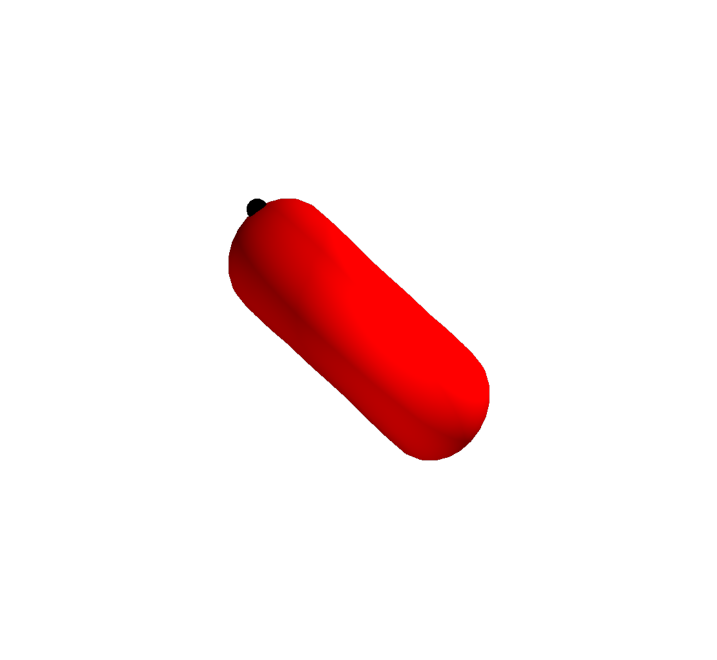
\includegraphics[trim=75 100 75 100, clip, width=\textwidth]{figures/tumble4000.png}\\
        $\dot{\gamma}t = 20$
    \end{minipage}%
    \phantomsubcaption
    \label{fig:tumble}
    \end{subfigure}
    \begin{subfigure}{\textwidth}
    \begin{minipage}{0.2\textwidth}
        \centering
        \topinset{(b)}{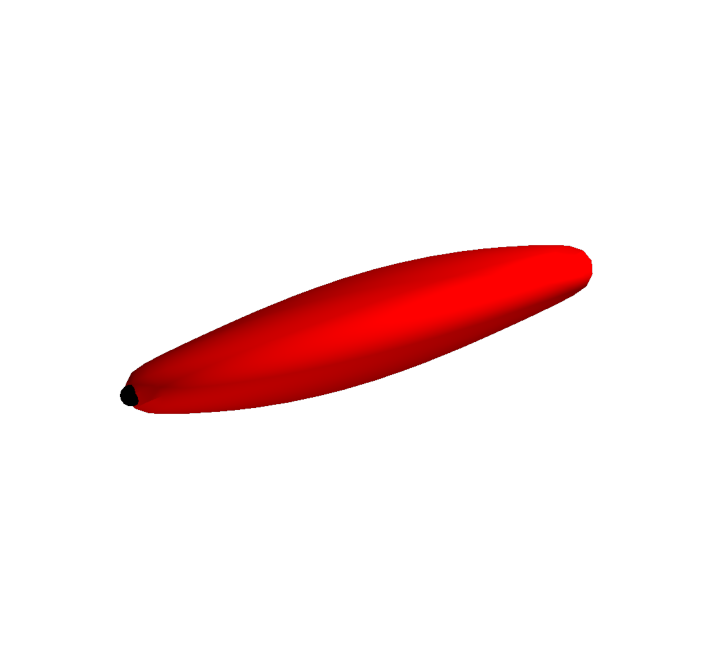
\includegraphics[trim=75 125 75 75, clip, width=\textwidth]{figures/tread0190.png}}{0.5cm}{0.25cm}\\
        $\dot{\gamma}t = 19$
    \end{minipage}%
    \begin{minipage}{0.2\textwidth}
        \centering
        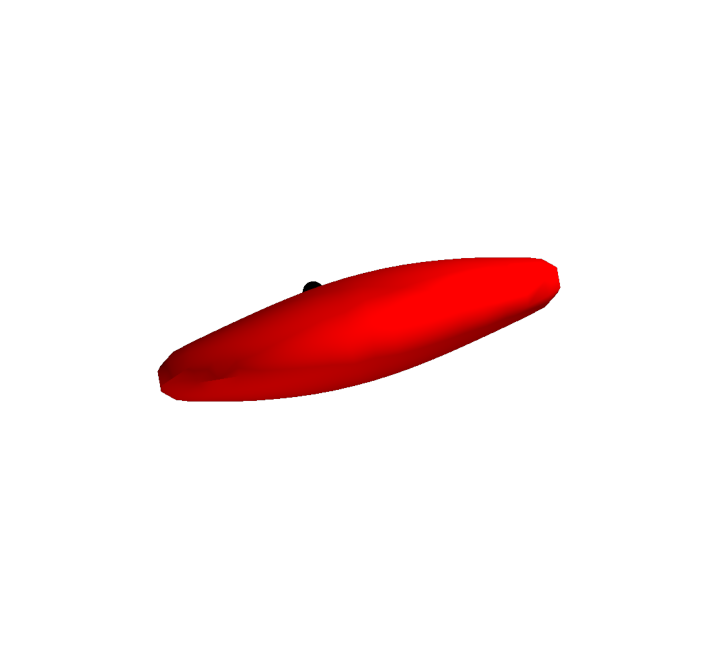
\includegraphics[trim=75 125 75 75, clip, width=\textwidth]{figures/tread0260.png}\\
        $\dot{\gamma}t = 26$
    \end{minipage}%
    \begin{minipage}{0.2\textwidth}
        \centering
        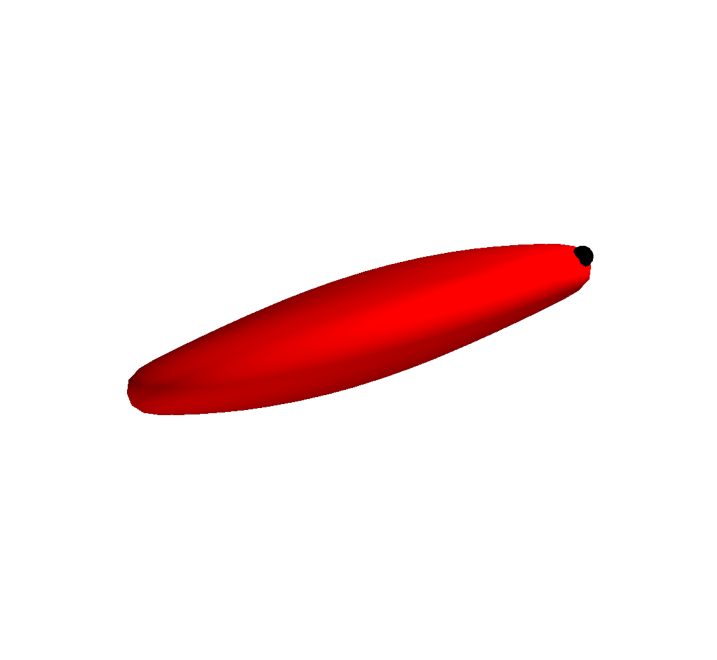
\includegraphics[trim=75 125 75 75, clip, width=\textwidth]{figures/tread0330.png}\\
        $\dot{\gamma}t = 33$
    \end{minipage}%
    \begin{minipage}{0.2\textwidth}
        \centering
        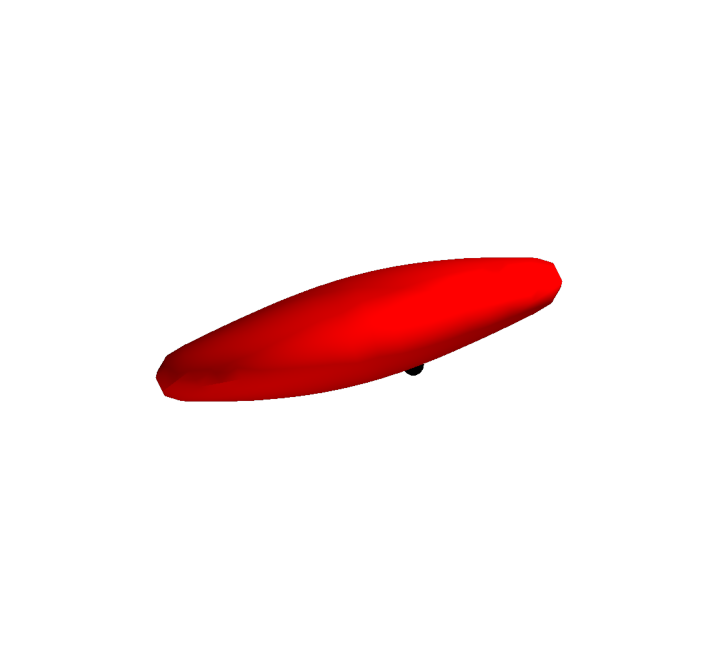
\includegraphics[trim=75 125 75 75, clip, width=\textwidth]{figures/tread0400.png}\\
        $\dot{\gamma}t = 40$
    \end{minipage}%
    \begin{minipage}{0.2\textwidth}
        \centering
        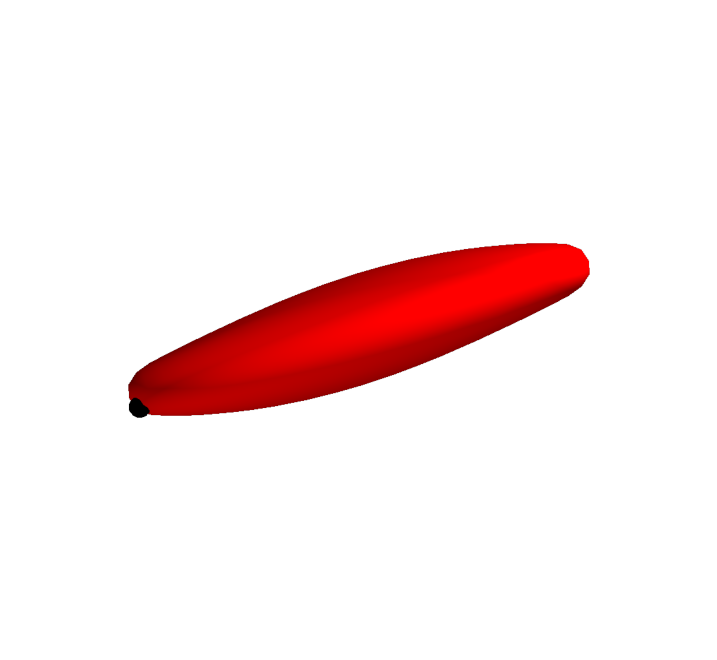
\includegraphics[trim=75 125 75 75, clip, width=\textwidth]{figures/tread0470.png}\\
        $\dot{\gamma}t = 47$
    \end{minipage}%
    \phantomsubcaption
    \label{fig:tread}
    \end{subfigure}
    \caption{%
        Our model RBC exhibits (a) a tumbling behavior under low shear
        ($\dot{\gamma} = 50\si{\per\second}$) conditions and (b) tank-treading under high
        shear ($\dot{\gamma} = 1000\si{\per\second}$) conditions.
    }%
    \label{fig:tumble-tread}
\end{figure}

RBCs are known to tumble end-over-end under low shear conditions. As shear rates
increase, the behavior transitions into a regime known as ``tank-treading'', in which
the cell takes on an elongated shape and the membrane {\XXX} rotates about its interior
fluid.

We place a single RBC with $\data\cardinality = 625$ and $\sample\cardinality = 2500$
in a $16\um\times16\um\times16\um$ domain, discretized to have $h = 0.4\um$. We use shear
rate $\dot{\gamma} = 50\si{\per\second}$ to capture the tumbling dynamics and
$\dot{\gamma} = 1000\si{\per\second}$ for tank-treading. One period of each is shown in
Figure~\ref{fig:tumble-tread}.
